\documentclass[a4paper,14pt,oneside,openany]{memoir}

%%% Задаем поля, отступы и межстрочный интервал %%%

\usepackage[left=10mm, right=15mm, top=20mm, bottom=20mm]{geometry} % Пакет geometry с аргументами для определения полей
\pagestyle{plain} % Убираем стандарные для данного класса верхние колонтитулы с заголовком текущей главы, оставляем только номер страницы снизу по центру
\parindent=1.25cm % Абзацный отступ 1.25 см, приблизительно равно пяти знакам, как по ГОСТ
\usepackage{indentfirst} % Добавляем отступ к первому абзацу
%\linespread{1.3} % Межстрочный интервал (наиболее близко к вордовскому полуторному) - тут вместо этого используется команда OnehalfSpacing*

%%% Задаем языковые параметры и шрифт %%%

\usepackage[english, russian]{babel}                % Настройки для русского языка как основного в тексте
\babelfont{rm}{Times New Roman}                     % TMR в качестве базового roman-щрифта

%%% Задаем стиль заголовков и подзаголовков в тексте %%%

\setsecnumdepth{subsection} % Номера разделов считать до третьего уровня включительно, т.е. нумеруются только главы, секции, подсекции
\renewcommand*{\chapterheadstart}{} % Переопределяем команду, задающую отступ над заголовком, чтобы отступа не было
\renewcommand*{\printchaptername}{} % Переопределяем команду, печатающую слово "Глава", чтобы оно не печалось
%\renewcommand*{\printchapternum}{} % То же самое для номера главы - тут не надо, номер главы оставляем
\renewcommand*{\chapnumfont}{\normalfont\bfseries} % Меняем стиль шрифта для номера главы: нормальный размер, полужирный
\renewcommand*{\afterchapternum}{\hspace{1em}} % Меняем разделитель между номером главы и названием
\renewcommand*{\printchaptertitle}{\normalfont\bfseries\centering\MakeUppercase} % Меняем стиль написания для заголовка главы: нормальный размер, полужирный, центрированный, заглавными буквами
\setbeforesecskip{20pt} % Задаем отступ перед заголовком секции
\setaftersecskip{20pt} % Ставим такой же отступ после заголовка секции
\setsecheadstyle{\raggedright\normalfont\bfseries} % Меняем стиль написания для заголовка секции: выравнивание по правому краю без переносов, нормальный размер, полужирный
\setbeforesubsecskip{20pt} % Задаем отступ перед заголовком подсекции
\setaftersubsecskip{20pt} % Ставим такой же отступ после заголовка подсекции
\setsubsecheadstyle{\raggedright\normalfont\bfseries}  % Меняем стиль написания для заголовка подсекции: выравнивание по правому краю без переносов, нормальный размер, полужирный

%%% Задаем параметры оглавления %%%

\addto\captionsrussian{\renewcommand\contentsname{Содержание}} % Меняем слово "Оглавление" на "Содержание"
\setrmarg{2.55em plus1fil} % Запрещаем переносы слов в оглавлении
%\setlength{\cftbeforechapterskip}{0pt} % Эта команда убирает интервал между заголовками глав - тут не надо, так красивее смотрится
\renewcommand{\aftertoctitle}{\afterchaptertitle \vspace{-\cftbeforechapterskip}} % Делаем отступ между словом "Содержание" и первой строкой таким же, как у заголовков глав
%\renewcommand*{\chapternumberline}[1]{} % Делаем так, чтобы номер главы не печатался - тут не надо
\renewcommand*{\cftchapternumwidth}{1.5em} % Ставим подходящий по размеру разделитель между номером главы и самим заголовком
\renewcommand*{\cftchapterfont}{\normalfont\MakeUppercase} % Названия глав обычным шрифтом заглавными буквами
\renewcommand*{\cftchapterpagefont}{\normalfont} % Номера страниц обычным шрифтом
\renewcommand*{\cftchapterdotsep}{\cftdotsep} % Делаем точки до номера страницы после названий глав
\renewcommand*{\cftdotsep}{1} % Задаем расстояние между точками
\renewcommand*{\cftchapterleader}{\cftdotfill{\cftchapterdotsep}} % Делаем точки стандартной формы (по умолчанию они "жирные")
\maxtocdepth{subsection} % В оглавление попадают только разделы первыхтрех уровней: главы, секции и подсекции

%%% Выравнивание и переносы %%%

%% http://tex.stackexchange.com/questions/241343/what-is-the-meaning-of-fussy-sloppy-emergencystretch-tolerance-hbadness
%% http://www.latex-community.org/forum/viewtopic.php?p=70342#p70342
\tolerance 1414
\hbadness 1414
\emergencystretch 1.5em                             % В случае проблем регулировать в первую очередь
\hfuzz 0.3pt
\vfuzz \hfuzz
%\dbottom
%\sloppy                                            % Избавляемся от переполнений
\clubpenalty=10000                                  % Запрещаем разрыв страницы после первой строки абзаца
\widowpenalty=10000                                 % Запрещаем разрыв страницы после последней строки абзаца
\brokenpenalty=4991                                 % Ограничение на разрыв страницы, если строка заканчивается переносом

%%% Объясняем компилятору, какие буквы русского алфавита можно использовать в перечислениях (подрисунках и нумерованных списках) %%%
%%% По ГОСТ нельзя использовать буквы ё, з, й, о, ч, ь, ы, ъ %%%
%%% Здесь также переопределены заглавные буквы, хотя в принципе они в документе не используются %%%

\makeatletter
    \def\russian@Alph#1{\ifcase#1\or
       А\or Б\or В\or Г\or Д\or Е\or Ж\or
       И\or К\or Л\or М\or Н\or
       П\or Р\or С\or Т\or У\or Ф\or Х\or
       Ц\or Ш\or Щ\or Э\or Ю\or Я\else\xpg@ill@value{#1}{russian@Alph}\fi}
    \def\russian@alph#1{\ifcase#1\or
       а\or б\or в\or г\or д\or е\or ж\or
       и\or к\or л\or м\or н\or
       п\or р\or с\or т\or у\or ф\or х\or
       ц\or ш\or щ\or э\or ю\or я\else\xpg@ill@value{#1}{russian@alph}\fi}
\makeatother

%%% Задаем параметры оформления рисунков и таблиц %%%

\usepackage{graphicx, caption, subcaption} % Подгружаем пакеты для работы с графикой и настройки подписей
\graphicspath{{images/}} % Определяем папку с рисунками
\captionsetup[figure]{font=small, width=\textwidth, name=Рисунок, justification=centering} % Задаем параметры подписей к рисункам: маленький шрифт (в данном случае 12pt), ширина равна ширине текста, полнотекстовая надпись "Рисунок", выравнивание по центру
\captionsetup[subfigure]{font=small} % Индексы подрисунков а), б) и так далее тоже шрифтом 12pt (по умолчанию делает еще меньше)
\captionsetup[table]{singlelinecheck=false,font=small,width=\textwidth,justification=justified} % Задаем параметры подписей к таблицам: запрещаем переносы, маленький шрифт (в данном случае 12pt), ширина равна ширине текста, выравнивание по ширине
\captiondelim{ --- } % Разделителем между номером рисунка/таблицы и текстом в подписи является длинное тире
\setkeys{Gin}{width=\textwidth} % По умолчанию размер всех добавляемых рисунков будет подгоняться под ширину текста
\renewcommand{\thesubfigure}{\asbuk{subfigure}} % Нумерация подрисунков строчными буквами кириллицы
%\setlength{\abovecaptionskip}{0pt} % Отбивка над подписью - тут не меняем
%\setlength{\belowcaptionskip}{0pt} % Отбивка под подписью - тут не меняем
\usepackage[section]{placeins} % Объекты типа float (рисунки/таблицы) не вылезают за границы секциии, в которой они объявлены

%%% Задаем параметры ссылок и гиперссылок %%% 

\usepackage{hyperref}                               % Подгружаем нужный пакет
\hypersetup{
    colorlinks=true,                                % Все ссылки и гиперссылки цветные
    linktoc=all,                                    % В оглавлении ссылки подключатся для всех отображаемых уровней
    linktocpage=true,                               % Ссылка - только номер страницы, а не весь заголовок (так выглядит аккуратнее)
    linkcolor=red,                                  % Цвет ссылок и гиперссылок - красный
    citecolor=red                                   % Цвет цитировний - красный
}

%%% Настраиваем отображение списков %%%

\usepackage{enumitem}                               % Подгружаем пакет для гибкой настройки списков
\renewcommand*{\labelitemi}{\normalfont{--}}        % В ненумерованных списках для пунктов используем короткое тире
\makeatletter
    \AddEnumerateCounter{\asbuk}{\russian@alph}     % Объясняем пакету enumitem, как использовать asbuk
\makeatother
\renewcommand{\labelenumii}{\asbuk{enumii})}        % Кириллица для второго уровня нумерации
\renewcommand{\labelenumiii}{\arabic{enumiii})}     % Арабские цифры для третьего уровня нумерации
\setlist{noitemsep, leftmargin=*}                   % Убираем интервалы между пунками одного уровня в списке
\setlist[1]{labelindent=\parindent}                 % Отступ у пунктов списка равен абзацному отступу
\setlist[2]{leftmargin=\parindent}                  % Плюс еще один такой же отступ для следующего уровня
\setlist[3]{leftmargin=\parindent}                  % И еще один для третьего уровня

%%% Счетчики для нумерации объектов %%%

\counterwithout{figure}{chapter}                    % Сквозная нумерация рисунков по документу
\counterwithout{equation}{chapter}                  % Сквозная нумерация математических выражений по документу
\counterwithout{table}{chapter}                     % Сквозная нумерация таблиц по документу

%%% Реализация библиографии пакетами biblatex и biblatex-gost с использованием движка biber %%%

\usepackage{csquotes} % Пакет для оформления сложных блоков цитирования (biblatex рекомендует его подключать)
\usepackage[%
backend=biber,                                      % Движок
bibencoding=utf8,                                   % Кодировка bib-файла
sorting=none,                                       % Настройка сортировки списка литературы
style=gost-numeric,                                 % Стиль цитирования и библиографии по ГОСТ
language=auto,                                      % Язык для каждой библиографической записи задается отдельно
autolang=other,                                     % Поддержка многоязычной библиографии
sortcites=true,                                     % Если в квадратных скобках несколько ссылок, то отображаться будут отсортированно
movenames=false,                                    % Не перемещать имена, они всегда в начале библиографической записи
maxnames=5,                                         % Максимальное отображаемое число авторов
minnames=3,                                         % До скольки сокращать число авторов, если их больше максимума
doi=false,                                          % Не отображать ссылки на DOI
isbn=false,                                         % Не показывать ISBN, ISSN, ISRN
]{biblatex}[2016/09/17]
\DeclareDelimFormat{bibinitdelim}{}                 % Убираем пробел между инициалами (Иванов И.И. вместо Иванов И. И.)
\addbibresource{biba.bib}                           % Определяем файл с библиографией

%%% Скрипт, который автоматически подбирает язык (и, следовательно, формат) для каждой библиографической записи %%%
%%% Если в названии работы есть кириллица - меняем значение поля langid на russian %%%
%%% Все оставшиеся пустые места в поле langid заменяем на english %%%

\DeclareSourcemap{
  \maps[datatype=bibtex]{
    \map{
        \step[fieldsource=title, match=\regexp{^\P{Cyrillic}*\p{Cyrillic}.*}, final]
        \step[fieldset=langid, fieldvalue={russian}]
    }
    \map{
        \step[fieldset=langid, fieldvalue={english}]
    }
  }
}

%%% Прочие пакеты для расширения функционала %%%

\usepackage{longtable,ltcaption}                    % Длинные таблицы
\usepackage{multirow,makecell}                      % Улучшенное форматирование таблиц
\usepackage{booktabs}                               % Еще один пакет для красивых таблиц
\usepackage{soulutf8}                               % Поддержка переносоустойчивых подчёркиваний и зачёркиваний
\usepackage{icomma}                                 % Запятая в десятичных дробях
\usepackage{hyphenat}                               % Для красивых переносов
\usepackage{textcomp}                               % Поддержка "сложных" печатных символов типа значков иены, копирайта и т.д.
\usepackage[version=4]{mhchem}                      % Красивые химические уравнения
\usepackage{amsmath} 

\usepackage[utf8]{inputenc}

\usepackage{amsthm}
\usepackage{amssymb}
\usepackage{enumerate}
\usepackage{stmaryrd}
\usepackage{cmll}
\usepackage{mathrsfs}
\usepackage{proof}
\usepackage{tikz}
\usepackage{multicol}
\usepackage{mathabx}
\usepackage{pdflscape}
\usepackage{listings}
\usepackage{xcolor}

\definecolor{codegreen}{rgb}{0,0.6,0}
\definecolor{codegray}{rgb}{0.5,0.5,0.5}
\definecolor{codepurple}{rgb}{0.58,0,0.82}
\definecolor{backcolour}{rgb}{0.95,0.95,0.92}

\lstdefinestyle{mystyle}{
    backgroundcolor=\color{backcolour},   
    commentstyle=\color{codegreen},
    keywordstyle=\color{magenta},
    numberstyle=\tiny\color{codegray},
    stringstyle=\color{codepurple},
    basicstyle=\ttfamily\footnotesize,
    breakatwhitespace=false,         
    breaklines=true,                 
    captionpos=b,                    
    keepspaces=true,                 
    numbers=left,                    
    numbersep=5pt,                  
    showspaces=false,                
    showstringspaces=false,
    showtabs=false,                  
    tabsize=2
}

\lstset{style=mystyle}

% Усовершенствование отображения математических выражений 

%%% Вставляем по очереди все содержательные части документа %%%

\begin{document}

\thispagestyle{empty}

\begin{center}

    Национальный исследовательский университет ИТМО\\
    Факультет информационных технологий и программирования\\
    Прикладная матеметика и информатика\\

    \vspace{20pt}

\end{center}

\vfill

\begin{center}
    \textbf {
    Методы оптимизации 
    } \\  
    Отчет по лабораторной работе №1
    
\end{center}

\vfill

\begin{flushright}

    \hfill {
    Работу \\
    выполняли: \\
    Кольченко Антон М32371 \\ 
    Гайнанов Ильдар М32371 \\ 
    Муфтиев Руслан М32331\\ 
    }
    \vspace{20pt}

    \hfill {
    Предподаватель: \\
    Казанков В.К.
    }

\end{flushright}

\vfill

\begin{center}
    Санкт-Петербург\\
    2023
\end{center}                                     % Титульник

\newpage % Переходим на новую страницу
\setcounter{page}{2} % Начинаем считать номера страниц со второй
\OnehalfSpacing* % Задаем полуторный интервал текста (в титульнике одинарный, поэтому команда стоит после него)

\tableofcontents*                                   % Автособираемое оглавление

\chapter*{Введение}
\addcontentsline{toc}{chapter}{Введение}
\label{ch:intro}
    \textbf{Постановка задачи:}

    \begin{enumerate}
        \item Реализация градиентного спуска с постоянным шагом (learning rate).
        \item Реализация метода одномерного поиска - метод дихотомии и градиентный спуск на его основе.
        \item Анализ траектории градиентного спуска на примере различных квадратичных
        функций.
        \item Для каждой функции:
        \begin{enumerate}[label=(\alph*)]
            \item исследовать сходимость градиентного спуска с постоянным шагом 
            и сравнить
            полученные результаты для выбранных функций;
            \item сравнить эффективность градиентного спуска с использованием одномерного поиска с точки зрения количества вычислений минимизируемой
            функции и ее градиентов;
            \item
            исследовать работу методов в зависимости от выбора начальной точки;
            \item исследовать влияние нормализации (scaling) на сходимость на примере масштабирования осей плохо обусловленной функции;
            \item нарисовать графики с линиями уровня и траекториямиметодов для каждого случая;
        \end{enumerate}
    
    \item Реализовать генератор случайных квадратичных функций $n$ переменных с числом обусловленности $k$.
    \item
    Исследовать зависимость числа итераций $T(n, k)$, необходимых градиентному
    спуску для сходимости в зависимости от размерности пространства $2 \leq n \leq 10^3$
    и числа обусловленности оптимизируемой функции $1 \leq k \leq 10^3$
    \item Проведение множественных экспериментов и для  полученния среднего  значения числа итераций.
    \item Реализовать одномерный поиск с учетом условий Вольфе и исследовать его эффективность, а также сравнить полученные результаты с реализованными ранее методами.
\end{enumerate}


\endinput                                     % Введение
\chapter{Теоретическая часть}
\label{ch:chap1}

    В этом разделе будут описаны все вычислительные схемы требующихся методов.

\section{Градиентный спуск с постоянным шагом (learning rate)}

    Принцип работы: 

    Суть метода градиентного спуска заключается в том, чтобы идти в направлении скорейшего спуска. Таким образом, за достаточное количество шагов можно дойти до локального минимума функции, если таковой существует.
    

    Вход: функция $f:\mathbb{R}^n \rightarrow \mathbb{R}$, стартовая точка $x = (x_1,x_2,...,x_n)$, точность $\varepsilon$, размер шага $\lambda$
    
    Выход: найденная точка локального минимума

    Алгоритм:
    \begin{enumerate}
        \item $x^{[k+1]} = x^{[k]} - \lambda\nabla f(x^{[k]})$.
        \item Повторять шаг 1, пока  $|x^{[k+1]} - x^{[k]}| > \varepsilon$.
    \end{enumerate}

    
    
\section{Метод дихотомии}

    Принцип работы:
    

    Вход: функция $f:\mathbb{R} \rightarrow \mathbb{R}$, стартовая точка $x$, точность $\varepsilon$, отрезок, на котором ищется минимум $[a ,b]$
    
    Выход: найденная точка локального минимума

    Алгоритм(для поиска минимума):
    \begin{enumerate}
        \item На каждом шаге процесса поиска делим отрезок $[a,b]$ пополам, $x = \frac{a + b}{2}$ - координата середины отрезка $[a,b]$.
        \item $x_1 := \frac{a + b}{2} + \delta, x_2 := \frac{a + b}{2} - \delta, \delta \in (0; \frac{a - b}{2})$
        \item Вычисляем значение функции $f$ в $x_1$ и $x_2$: 

        $F_1 = f(x_1), F_2 = f(x_2)$

        \item Сравниваем $F_1$ и $F_2$ и выбираем отрезок для дальнейшего рассмотрения:
        \begin{itemize}
            \item Если $F_1 < F_2$ , то отбрасываем отрезок $[x_2,b]$, тогда $b = x_2$, рассматриваем $[a, x_2]$.
            \item Иначе рассматриваем $[x_1, b]$.
        \end{itemize}

        \item Деление отрезка $[a,b]$ продолжается до тех пор, пока его длина не станет меньше заданной точности $\varepsilon$, т.е. $|b - a| \leq\varepsilon$
    \end{enumerate}


\section{Градиентный спуск на основе метода дихотомии}

    Принцип работы:

жюдююжд    Принцип работы данной модификации абсолютно схож с вычислительной схемой обычного градиентного спуска, кроме одного пункта. Вместо того, чтобы прыгать на опрделенный шаг, для начала мы найдем точку минимума функции на одномерном отрезке $[x^{[k]}, x^{[k]} + \lambda\nabla f(x^{[k]})]$. Этот прием поможет сходиться с ответом в некоторых случаях за меньшее количество итераций, но количество процессорного времени, затраченного алгоритмом, будет выше, чем для обычного градиентного спуска для достижения высокой точности (будет проиллюстрировано в практической части).

    Алгоритм:
    
    Вход: функция $f:\mathbb{R}^n \rightarrow \mathbb{R}$, стартовая точка $x$, точность $\varepsilon$, размер шага $\lambda$
    \begin{enumerate}
        \item $x^{'[k]} = x^{[k]} - \lambda\nabla f(x^{[k]})$.
        \item Найти с помощью метода дихотомии локальный минимум на отрезке $[x^{[k]}, x^{'[k]}]$. Обозначим этот минимум как $x^{[k + 1]}$
        \item Повторять шаги 1-2, пока  $|x^{[k+1]} - x^{[k]}| > \varepsilon$.
    \end{enumerate}


\section{Оптимизация градиентного спуска с помощью условия Вольфе}

    Принцип работы:
    У градиентного спуска с постоянным шагом есть недостаток: если алгоритм находится слишком близко к точке минимума, то с постоянным шагом алгоритм может "перескочить" через точку экстремума, что приведет к тому, что будет затрачено больше итераций, чем нужно. Поэтому стоит ввести механизм изменения размера шага. В данном случае мы будем использовать критерий Вольфе.

    Определение критерия Вольфе:

    $p$ - направление, в котором мы хотим изменить $x$, в случае градиентного спуска - антиградиент функции в точке $x$

    $f(x + \alpha p) \leq f(x) + c_1 \alpha \nabla f^T p$

    $|\nabla f(x + \alpha p)^T p| \geq |c_2 \nabla f^T p|$

    $0 < c_1 < c_2 < 1$, $c_1$ близко к $0$, $c_2$ близко к $1$

    
    
    Вход: функция $f:\mathbb{R}^n \rightarrow \mathbb{R}$, стартовая точка $x$, точность $\varepsilon$, начальный шаг $\alpha_0$

    Выход: найденная точка локального минимума

    Алгоритм:
    \begin{enumerate}
        \item $\alpha = \alpha_0$
        \item Уменьшаем $\alpha$ до того момента, пока критерий Вольфе не начнет исполняться.
        \item $x^{[k + 1]} = x^{[k]} - \alpha\nabla f(x^{[k]})$.
        \item Повторять шаги, пока  $|x^{[k+1]} - x^{[k]}| > \varepsilon$.
    \end{enumerate}
    

\endinput                                     % Первая глава
\chapter{Практическая часть}
\label{ch:chap2}

\section{Реализация градиентного спуска с постоянным шагом (learning rate)}
\label{sec:fig}

\textbf{Сейчас и в последующем будем считать, что $\varepsilon = 10^{-6}$, в крайних случаях, если значение изменится, об этом будет сказано}

\begin{lstlisting}[language=Python, caption=Функция градиента]
import numpy as np
import scipy
import matplotlib.pyplot as plt

eps = 1e-6

def grad(f,x):
    h = 1e-6
    l = f(x[:,np.newaxis] + h * np.eye(x.size))
    r = f(x[:,np.newaxis] - h * np.eye(x.size));
    return (l - r)/(2*h)
\end{lstlisting}

\begin{lstlisting}[language=Python, caption=Градиентный спуск]
def gradient_descent(f,x,lr,lim=2000):
    points = []
    points.append(x)
    while f(x) - f(x - lr * (g := grad(f,x))) > eps:
        x = x - lr * g
        points.append(x)
        if len(points) > lim:
          return np.array([])
    return np.array(points)
\end{lstlisting}

\begin{lstlisting}[language=Python]
def f(x):
    return (x[0] - 2) ** 2 + (x[1] + 3) ** 2
t = np.linspace(-10,10,100)
X, Y = np.meshgrid(t,t)
ax = plt.figure().add_subplot(projection='3d')
ax.set_xlabel("x")
ax.set_ylabel("y")
ax.set_zlabel("f(x,y)")
ax.plot_surface(X, Y, f(np.stack((X, Y))))
\end{lstlisting}

\newpage

\begin{figure}[ht]
    \centering
    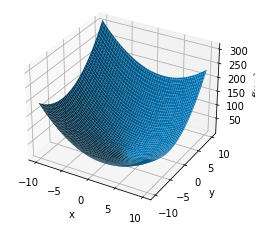
\includegraphics[width=0.5\textwidth]{images/gd1.png}
    \caption{Функция и ее график}
    \label{fig:gd1}
\end{figure}

\begin{lstlisting}[language=Python]
lr = 0.1
x = np.array([-1,1])
points = gradient_descent(f,x,lr)
print("x = ",points[-1])
print("f(x) = ",f(points[-1]))
plt.plot(points[:, 0], points[:, 1], 'o-')
plt.contour(X, Y, f([X, Y]), levels=sorted([f(p) for p in points]))
\end{lstlisting}

\begin{figure}[ht]
    \centering
    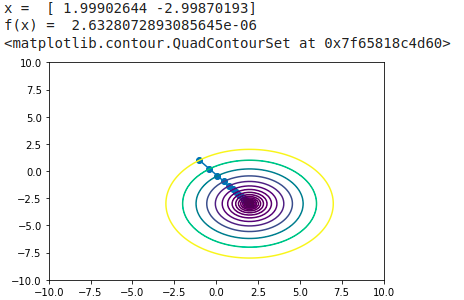
\includegraphics[width=0.5\textwidth]{images/gd2.png}
    \caption{Графическая интерпретация итераций алгоритма}
    \label{fig:gd2}
\end{figure}

\newpage

\section{Реализация градиентного спуска на основе одномерного поиска}

\subsection{Метод дихотомии}

\begin{lstlisting}[language=Python]
def f(x):
    return (x / 16 - 1) ** 2 * (2 * x ** 3 - 15 * x) - x ** 2

alpha = 12
beta = 19
t = np.linspace(alpha,beta,10000)
y = (0.2 * t - 1) * (0.2 * t - 6) ** 3 + 70
plt.plot(t,f(t))
plt.xlabel("x")
plt.ylabel("f(x)")
plt.show()
\end{lstlisting}

\begin{figure}[ht]
    \centering
    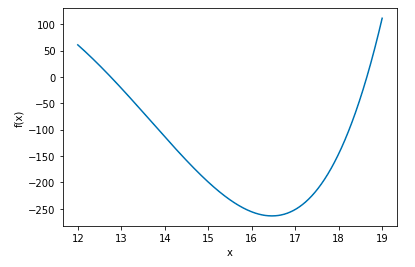
\includegraphics[width=0.5\textwidth]{images/t21.png}
    \caption{Берем произвольную функцию одного переменного}
    \label{fig:t21}
\end{figure}

\begin{lstlisting}[language=Python]
x = [alpha,beta]

points = []
points.append(x[::])

# Dichotomy algorithm
while (x[1] - x[0]) > eps:
    delta = eps / 2
    x1 = (x[0] + x[1]) / 2 - delta / 2
    x2 = (x[0] + x[1]) / 2 + delta / 2
    if f(x1) < f(x2):
        x[1] = x2
    else: 
        x[0] = x1
    points.append(x[::])

points = np.array(points)

ax1 = plt.subplot(1, 2, 1)
ax2 = plt.subplot(1, 2, 2)
ax1.set_xlabel("x")
ax2.set_xlabel("x")
ax1.set_ylabel("f(x)")
ax2.set_ylabel("f(x)")
pos1 = ax2.get_position()
ax2.set_position([pos1.x0 + 0.1,
                  pos1.y0,
                  pos1.width,
                  pos1.height])
ax1.scatter((points[::,0] + points[::,1]) / 2,f((points[::,0] + points[::,1]) / 2,), color='red')
ax1.plot(t,f(t))
ax2.plot(f((points[::,0] + points[::,1]) / 2))
\end{lstlisting}

\begin{figure}[ht]
    \centering
    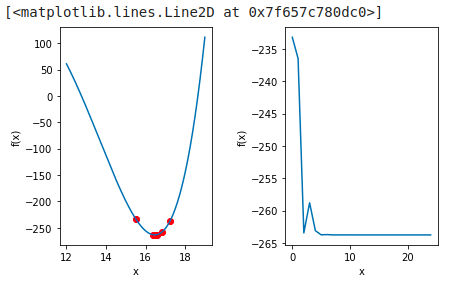
\includegraphics[width=0.5\textwidth]{images/t22.png}
    \caption{Пример работы дихотомии}
    \label{fig:t222}
\end{figure}

\newpage

\subsection{Модифицированный градиентный спуск}

\begin{lstlisting}[language=Python]
def dichotomy(f,a,b):
    x = np.array([a,b])
    while dist(x[0],x[1]) > eps:
        delta = (x[1] - x[0]) / 2
        x1 = (x[0] + x[1]) / 2 - delta / 2
        x2 = (x[0] + x[1]) / 2 + delta / 2
        new_x = np.copy(x)
        if f(x1) < f(x2):
            new_x[1] = x2
        else:
            new_x[0] = x1
        x = new_x

    return (x[0] + x[1]) / 2
    
def gradient_descent_with_dichotomy(f,x,lr,lim=2000):
    points = []
    points.append(x)
    while f(x) - f(x - lr * (g := grad(f,x))) > eps:
        x = dichotomy(f,x,x - lr * g)
        points.append(x)
        if len(points) > lim:
          return np.array([])
    return np.array(points)
\end{lstlisting}
\newpage
Функция №1

$f(x,y) = \frac{1}{50}x^2 + 50y^2$

\begin{figure}[ht]
    \centering
    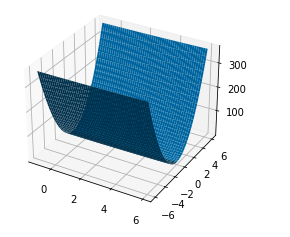
\includegraphics[width=0.5\textwidth]{images/g10.png}
    \caption{График функции}
    \label{fig:g10}
\end{figure}

\begin{figure}[ht]
    \centering
    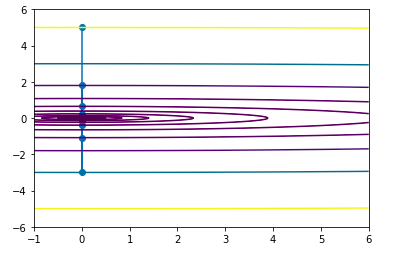
\includegraphics[width=0.5\textwidth]{images/g11.png}
    \caption{Работа ГС с постоянным шагом}
    \label{fig:g11}
\end{figure}

\begin{figure}[ht]
    \centering
    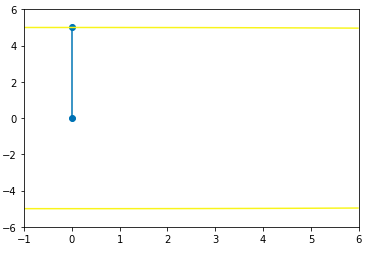
\includegraphics[width=0.5\textwidth]{images/g12.png}
    \caption{Работа ГС на основе дихотомии}
    \label{fig:g12}
\end{figure}

\newpage

Функция №2

$f(x,y) = \frac{1}{10}x^2 + 10y^2$

\begin{figure}[ht]
    \centering
    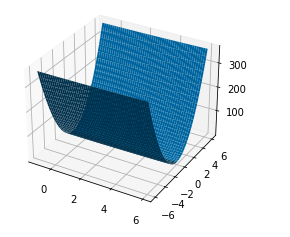
\includegraphics[width=0.5\textwidth]{images/g10.png}
    \caption{График функции}
    \label{fig:g10}
\end{figure}

\begin{figure}[ht]
    \centering
    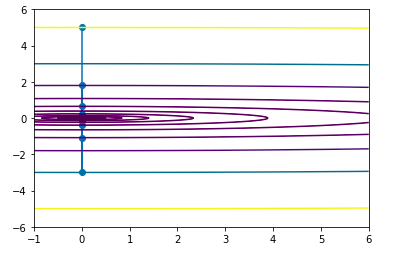
\includegraphics[width=0.5\textwidth]{images/g11.png}
    \caption{Работа ГС с постоянным шагом}
    \label{fig:g11}
\end{figure}

\begin{figure}[ht]
    \centering
    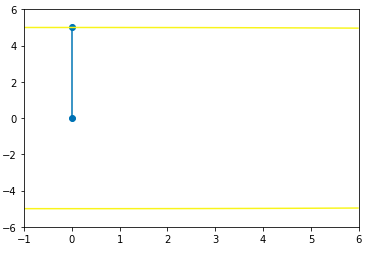
\includegraphics[width=0.5\textwidth]{images/g12.png}
    \caption{Работа ГС на основе дихотомии}
    \label{fig:g12}
\end{figure}

\newpage

Функция №3

$f(x,y) = (x^2 + y - 11)^2 + (x + y^2 - 7)^2$

\begin{figure}[ht]
    \centering
    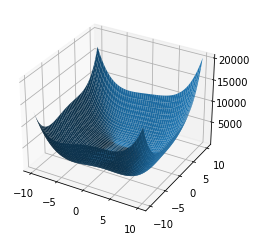
\includegraphics[width=0.5\textwidth]{images/g30.png}
    \caption{График функции}
    \label{fig:g30}
\end{figure}

\begin{figure}[ht]
    \centering
    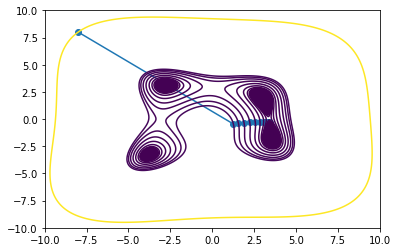
\includegraphics[width=0.5\textwidth]{images/g31.png}
    \caption{Работа ГС с постоянным шагом}
    \label{fig:g31}
\end{figure}

\newpage

\begin{figure}[ht]
    \centering
    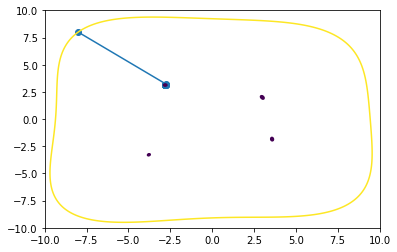
\includegraphics[width=0.5\textwidth]{images/g32.png}
    \caption{Работа ГС на основе дихотомии}
    \label{fig:g32}
\end{figure}

\begin{landscape}
\section{Дополнительные исследования}
\begin{vplace}[1.0]
\begin{figure}[ht]
    \centering
    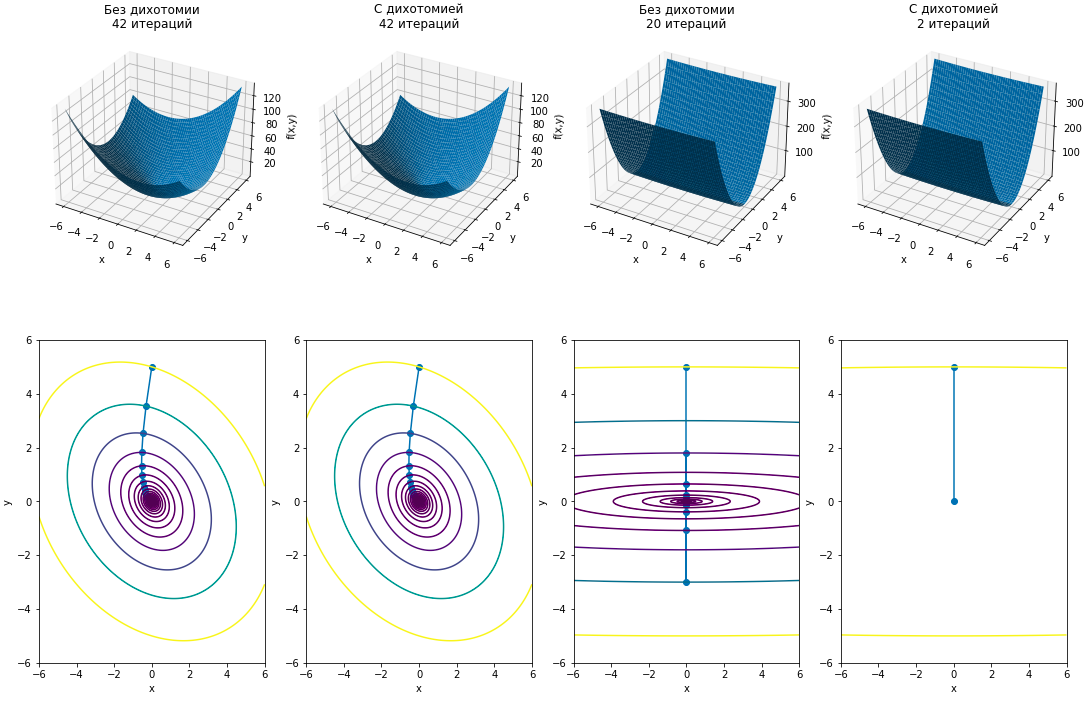
\includegraphics[width=1.0\textwidth]{images/4a.png}
    \caption{Сравнение количества итераций алгоритмов ГС}
    \label{fig:4a}
\end{figure}
\end{vplace}
\end{landscape}


Количество вызовов функции и подсчетов градиентов для данных случаев:
    \begin{enumerate}
    \item Вызовы функции: 132 \\
    Подсчеты градиента: 33
    \item Вызовы функции: 2230 \\
    Подсчеты градиента: 33
    \item Вызовы функции: 80 \\
    Подсчеты градиента: 20
    \item Вызовы функции: 120 \\
    Подсчеты градиента: 2
    \end{enumerate}
\begin{landscape}
\begin{vplace}[1.0]
\begin{figure}[ht]
    \centering
    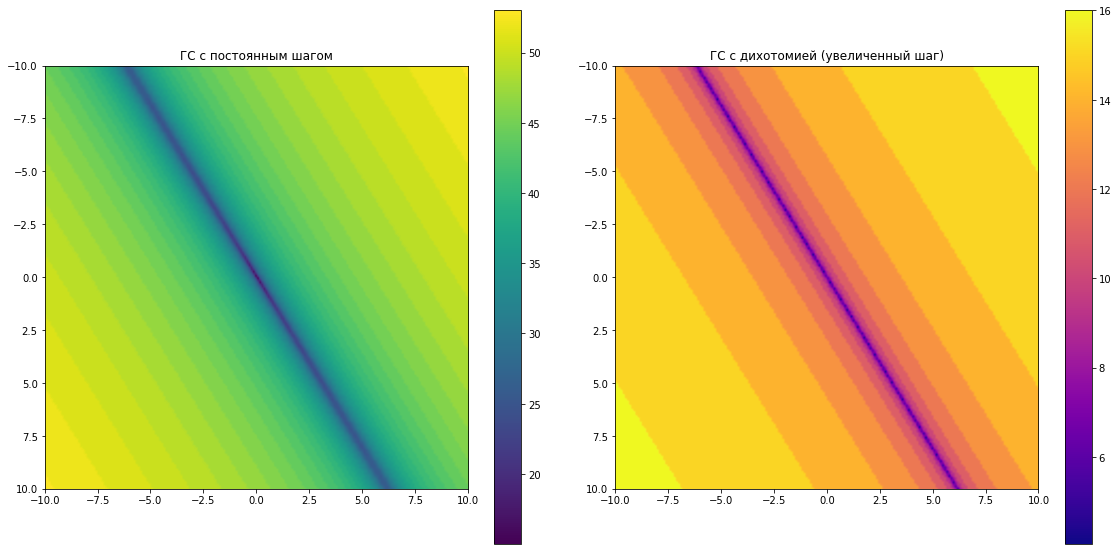
\includegraphics[width=1.5\textwidth]{images/4c.png}
    \caption{Количество итераций алгоритмов ГС в зависимости от выбора начальной точки}
    \label{fig:4c}
\end{figure}
\end{vplace}
\end{landscape}
\begin{landscape}
\begin{vplace}[1.0]
\begin{figure}[ht]
    \centering
    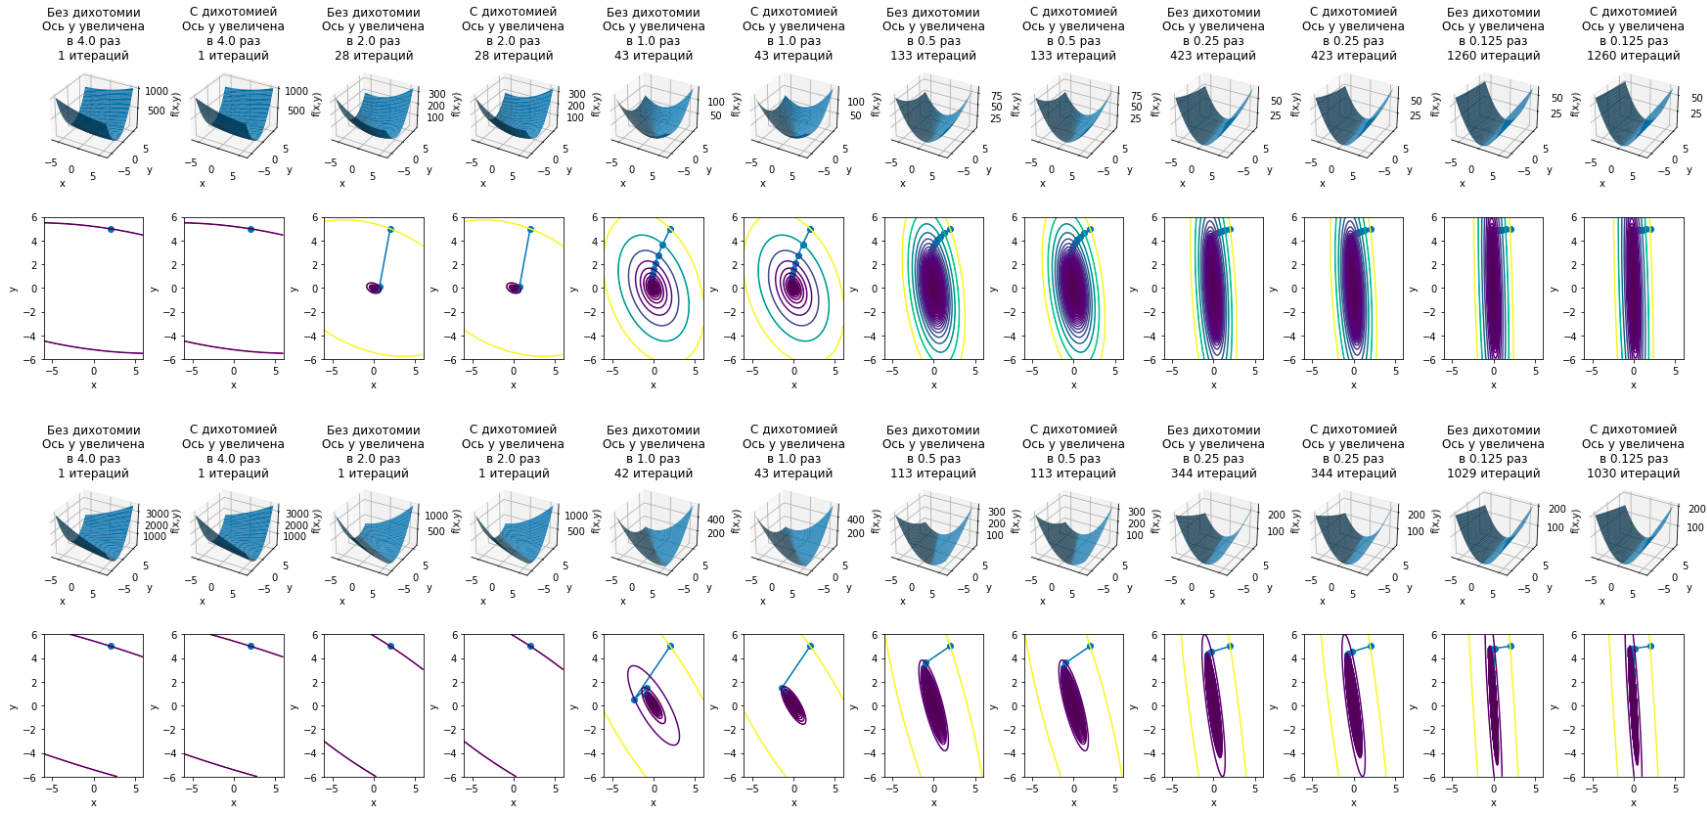
\includegraphics[width=1.5\textwidth]{images/4d.png}
    \caption{Количество итераций алгоритмов ГС в зависимости от масштабирования осей}
    \label{fig:4d}
\end{figure}
\end{vplace}
\end{landscape}
\section{Анализ градиентного спуска и его модификации на основе дихотомии}

Эффективность градиентного спуска сильно зависит от выбора шага. Если шаг будет слишком большой, то алгоритм градиентного спуска может "перескочить" точку минимума (См. графики функций 1 и 2), что приведет к лишним итерациям алгоритма, а в крайне плохих плохих случаях к тому, что градиентный спуск не будет сходиться.

Модификация градиентного спуска с использованием дихотомии позволяет алгоритму сходиться в таких случаях, причем значительно быстрее, чем сходится градиентный спуск с постоянным шагом. Однако если шаг слишком мал, то результат модифицированного алгоритма не будет отличаться от обычного градиентного спуска ничем, кроме времени исполнения, которое у модифицированного алгоритма будет значительно больше (см. дополнительное исследование 1).

На примере функции №3 мы можем заметить, что обычный и модифицированый градиентный спуск могут вернуть различные точки минимума. (В данном случае это не является проблемой, так как приведенная функция имеет 4 точки минимума с равными значениями функции в них.)

Если шаг слишком маленький, то это так же может приводить к лишним итерациям алгоритма. В дополнительном исследовании 2 в каждом тесте не изменялись никакие переменные, кроме точки запуска алгоритма, которая отдалялась от точки минимума, что приводило к увеличению времени исполнения алгоритмов. 

Ускорить выполнение можно с помощью нормализации осей функции. По результатам дополнительного исследования можно увидеть, что существуют случаи, когда методы ГС не сходятся или сходятся за очень большое количество итераций, и это можно исправить с помощью нормализации.

\section{Реализация генератора квадратичных функций $n$ переменных с числом обусловленности $k$}

\begin{lstlisting}[language=Python]
# Quadratic function generation
def gen_f(n,k):
    m = np.random.rand(n, n) * 2
    Q, _ = np.linalg.qr(m)
    D = np.diag(np.array([k] + [1] * (n - 1)))

    result = Q @ D @ np.linalg.inv(Q)
    def f_impl(x):
        return x.T @ result @ x

    def f(x):
        return np.apply_along_axis(f_impl, 0, x)
        
    return f

def gen_f_poly(n,k):
    m = np.random.rand(n, n) * 2
    Q, _ = np.linalg.qr(m)
    D = np.diag(np.array([k] + [1] * (n - 1)))

    result = Q @ D @ np.linalg.inv(Q)
    
    parts = []
    for i in range(n):
      for j in range(n):
        x = f'x{i}^2' if i == j else f'x{i}*x{j}'
        parts.append(f'{result[i][j]}*{x}')

    return ' + '.join(parts)

gen_f_poly(2, 1000)
\end{lstlisting}

\begin{figure}[ht]
    \centering
    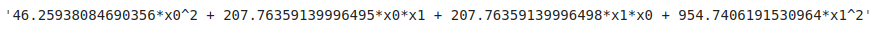
\includegraphics[width=0.5\textwidth]{images/gen1.png}
    \caption{Генератор функций, вывод сгенерированной функции в виде полинома}
    \label{fig:gen1}
\end{figure}

\begin{figure}[ht]
    \centering
    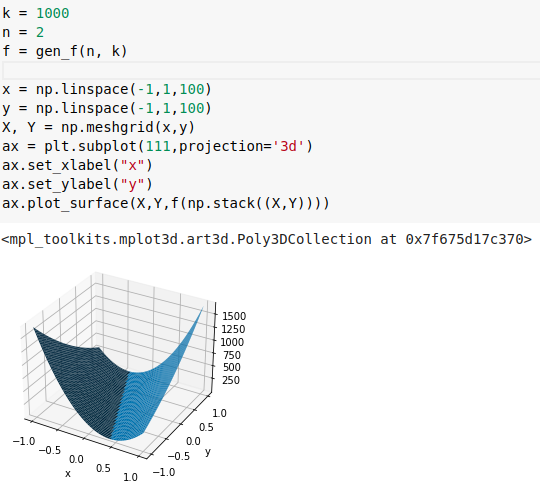
\includegraphics[width=0.5\textwidth]{images/gen2.png}
    \caption{Пример работы генерации функции для $n=2$ и $k=1000$}
    \label{fig:gen2}
\end{figure}

\section{Исследование зависимости числа итераций, необходимых градиетному спуску для сходимости}

\begin{figure}[ht]
    \centering
    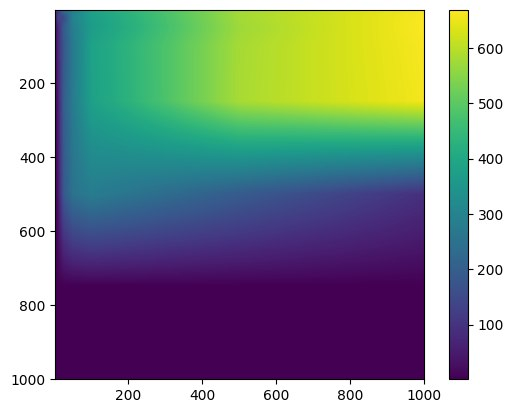
\includegraphics[width=0.5\textwidth]{images/task6-7.jpg}
    \caption{Тепловая карта значений $T(n,k)$ (по горизонтали - n, по вертикали - k)}
    \label{fig:task6-7}
\end{figure}

\section{Реализация одномерного поиска с условием Вольфе}

\begin{lstlisting}[language=Python, caption=Проверка условия Вольфе]
def check_wolfe(f, x, alpha, dir, c1=0.1, c2=0.9):
  gx = grad(f, x)
  cond1 = f(x + alpha*dir) <= f(x) + alpha * c1 * np.dot(dir, gx)
  cond2 = abs(np.dot(dir, grad(f, x + alpha * dir))) <= abs(c2 * np.dot(dir, gx))
  return cond1 and cond2
\end{lstlisting}


\begin{lstlisting}[language=Python, caption=Нахождение коэффициента для условия Вольфе и градиентный спуск на основе условия Вольфе]
def find_wolfe(f, x, dir):
    m = mk = 1
    start_alpha = 0.5
    for m in range(1, 20):
        alpha = start_alpha ** m
        if check_wolfe(f, x, alpha, dir):
          mk = m
          break
    return start_alpha ** mk

def gradient_descent_wolfe(f,x,lim=2000):
    points = []
    points.append(x)
    g = grad(f, x)
    if (np.linalg.norm(g) < 1e-6):
      return np.array(points)
    alpha = find_wolfe(f, x, -g)
    while f(x) - f(x - alpha * g) > 1e-6:
        x = x - alpha * g
        points.append(x)
        if len(points) > lim:
          return np.array([])
        g = grad(f, x)
        if (np.linalg.norm(g) < 1e-6):
          return np.array(points)
        alpha = find_wolfe(f, x, -g)
    return np.array(points)
\end{lstlisting}



\begin{landscape}
\begin{vplace}[1.0]    
\begin{figure}[ht]
    \centering
    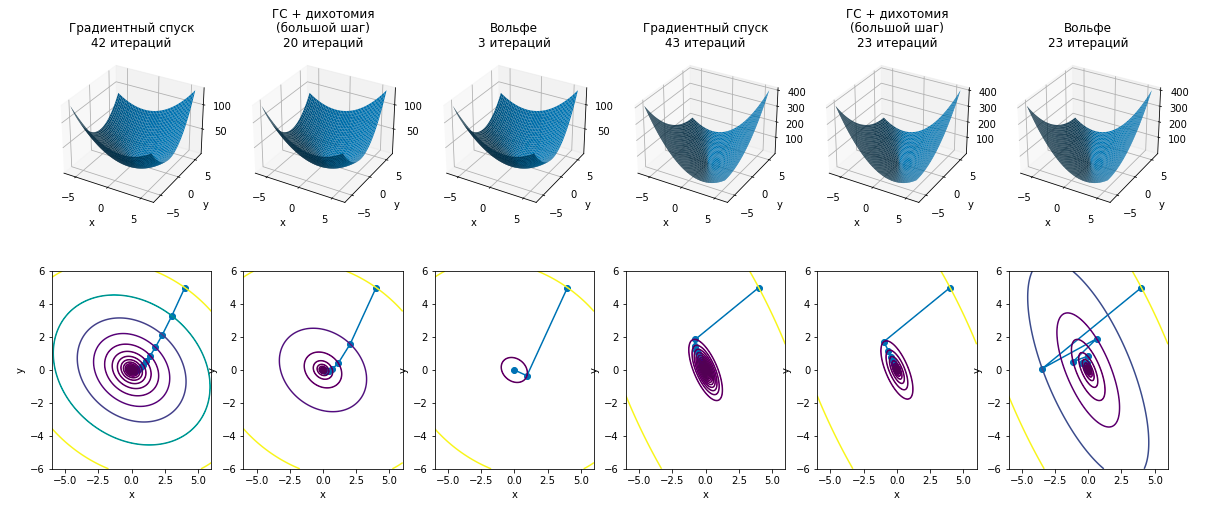
\includegraphics[width=1.5\textwidth]{images/w4.png}
    \caption{Сравнение методов}
    \label{fig:w4}
\end{figure}
\end{vplace}
\end{landscape}

\endinput                                     % Вторая глава
\chapter{Выводы}
\label{ch:tab}

Итак, в данной работе было рассмотрено несколько вариаций реализации метода градиентного спуска для нахождения наиболее оптимального(минимального) значения функции нескольких переменных. Как оказалось, у различных методов имеются свои сильные и слабые стороны. Кроме того, различные модификации алгоритма в некоторых случаях ускоряют процесс поиска, а других, наоборот.

    Как оказалось, на сходимость методов градиентного спуска сильно влияет длина шага. Мы рассмотрели метод дихотомии и критерий Вольфе, с помощью которых мы можем подобрать более удачную длину шага. Стандартный градиентный спуск плохо справляется на некоторых функциях. В большинстве случаев градиентный спуск с использованием дихотомии работает за такое же количество итераций, но есть функции, на которых это количество уменьшается в разы. Градиентный спуск же с использованием критерия Вольфе показал себя как достаточно универсальный метод, работающий в большинстве случаев быстрее стандартного градиентного спуска.

    Нами так же было рассмотрено влияние различных параметров на скорость сходимости методов градиентного спуска. Мы сделали следующие выводы:
    \begin{itemize}
        \item С ростом числа обусловленности алгоритмы градиентного спуска сходятся быстрее.
        \item С ростом размерности функции алгоритмы градиентного спуска требуют больше итераций для завершения.
    \end{itemize}

\endinput                                     % Третья глава

\printbibliography[title=Список использованных источников] % Автособираемый список литературы

\end{document}